\documentclass[serif, aspectratio=169]{beamer}
\usepackage[T1]{fontenc} 
\usepackage{fourier}
\usepackage{hyperref}
\usepackage{latexsym,amsmath,xcolor,multicol,booktabs,calligra}
\usepackage{booktabs} % For better table formatting
\usepackage{graphicx,pstricks,listings,stackengine}
\usepackage{listings}
\usepackage{array} 
\usepackage{colortbl}

\author{Dr.Hajialiasgari}
\title{Machine Learning}
\institute{
    Tehran University \\
    Of\\
    Medical Science
}
\date{\small \today}
\usepackage{UoWstyle}

% Define custom colors and styles for listings
\definecolor{deepblue}{rgb}{0,0,0.5}
\definecolor{deepred}{RGB}{153,0,0}
\definecolor{deepgreen}{rgb}{0,0.5,0}
\definecolor{halfgray}{gray}{0.55}

\lstset{
    basicstyle=\ttfamily\small,
    keywordstyle=\bfseries\color{deepblue},
    emphstyle=\ttfamily\color{deepred},
    stringstyle=\color{deepgreen},
    numbers=left,
    numberstyle=\small\color{halfgray},
    rulesepcolor=\color{red!20!green!20!blue!20},
    frame=shadowbox,
}

\begin{document}

\begin{frame}
    \titlepage
    \vspace*{-0.6cm}
    \begin{figure}[htpb]
        \begin{center}
            \includegraphics[keepaspectratio, scale=0.05]{Tumsl-logo.png}
        \end{center}
    \end{figure}
\end{frame}

\begin{frame}    
\tableofcontents[sectionstyle=show, subsectionstyle=show/shaded/hide, subsubsectionstyle=show/shaded/hide]
\end{frame}

\section{Introduction}

\subsection{Ensemble Learning}

\begin{frame}{Ensemble Learning}
    Ensemble learning is a technique that combines multiple models to improve predictive performance.
    \begin{itemize}
        \item \textbf{Improved Accuracy} – Combining multiple models results in better approximations.
        \item \textbf{Reduced Overfitting} – Averaging multiple models minimizes overfitting.
        \item \textbf{Increased Stability} – Reduces sensitivity to small variations in data.
    \end{itemize}
\end{frame}

\begin{frame}{How Ensemble Learning Work}
    \centering
    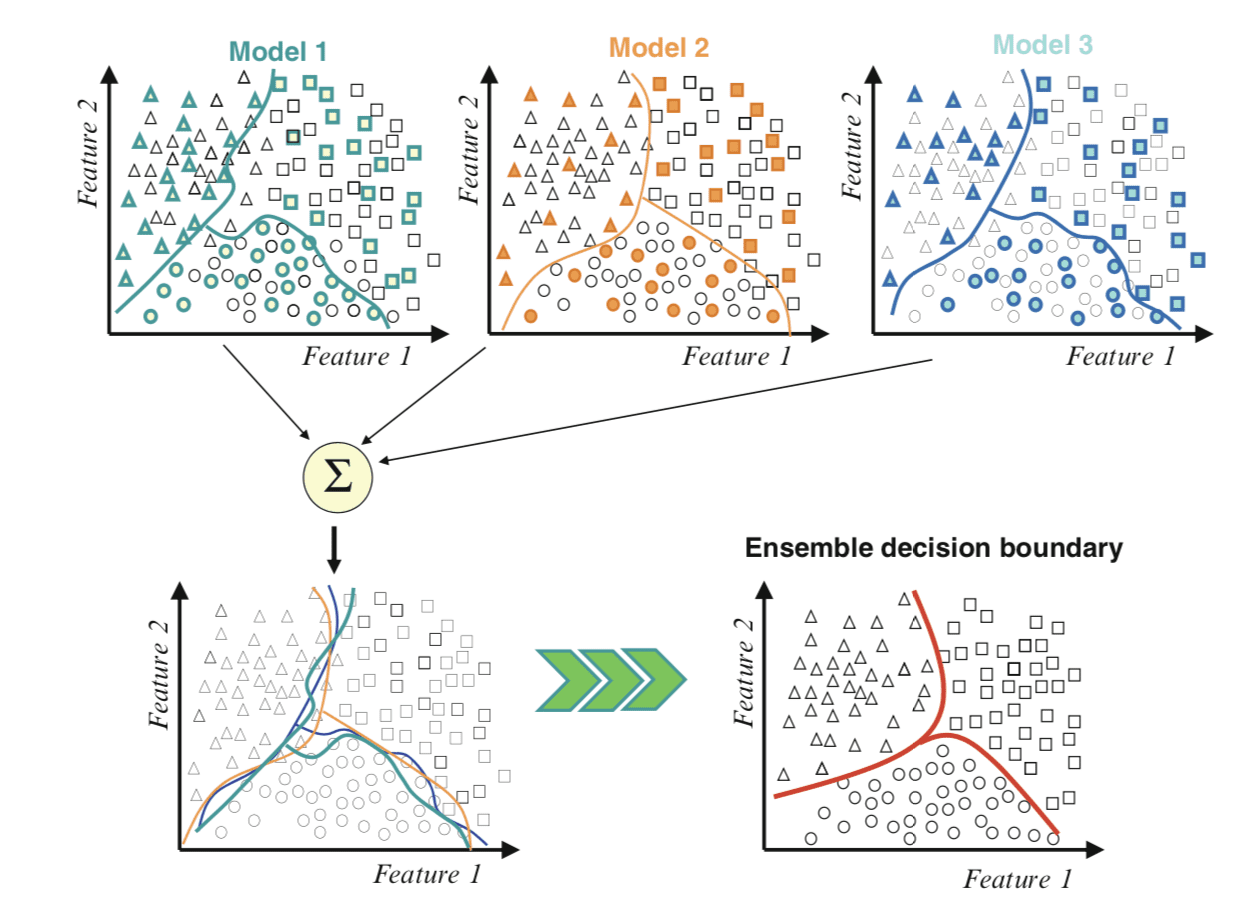
\includegraphics[width=0.7\textwidth]{Ensemble-Learning.png}
\end{frame}

\subsection{Ensemble Methodes}

\begin{frame}{Parallel Ensemble Methods}
    In parallel ensemble methods, models are trained independently, and their outputs are combined.
    Examples include:
    \begin{itemize}
        \item Bagging (Bootstrap Aggregating)
        \item Random Forest
    \end{itemize}
    These methods aim to reduce variance.
\end{frame}

\begin{frame}{Sequential Ensemble Methods}
    In sequential ensemble methods, models are trained in sequence, with each model correcting the errors of the previous one.
    Examples include:
    \begin{itemize}
        \item Boosting (AdaBoost, Gradient Boosting, XGBoost)
        \item Stacking (Stacked Generalization)
    \end{itemize}
    These methods aim to reduce bias.
\end{frame}

\begin{frame}{Sequential Vs Parallel}
    \centering
    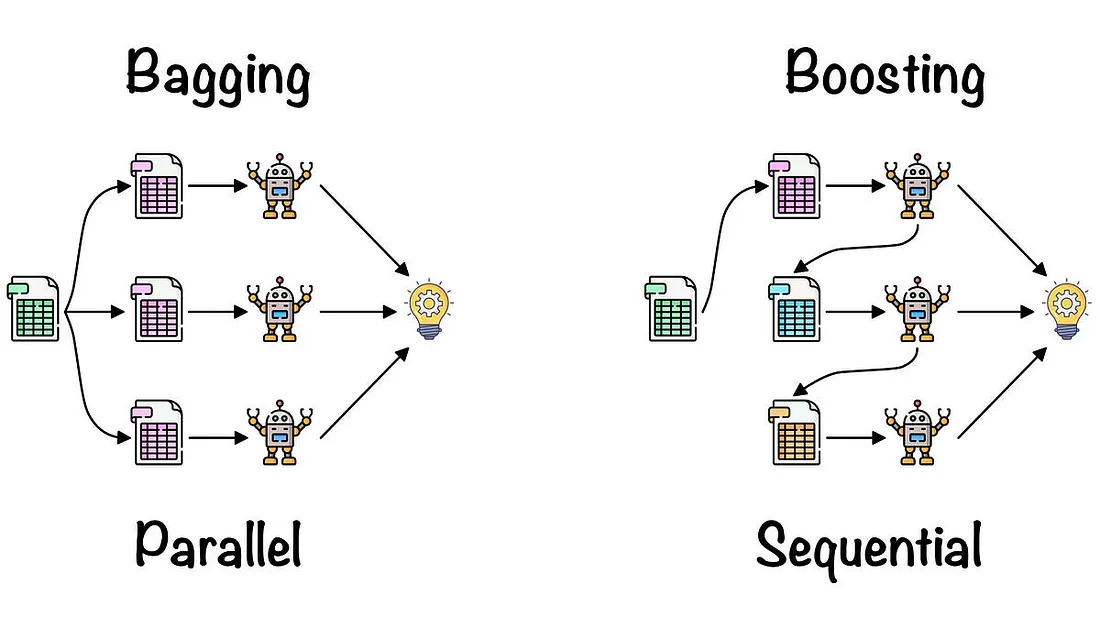
\includegraphics[width=0.9\textwidth]{Parallel-vs-Sequential.jpg}
\end{frame}

\section{Bagging}

\subsection{Basic idea and Algorithm}

\begin{frame}{Basic Idea:}
    \begin{itemize}
        \item Bagging is an ensemble learning technique designed to reduce variance and improve stability.
        \item It creates multiple independent models by training them on different subsets of the original dataset.
        \item The predictions of all models are then combined to form a final output.
    \end{itemize}
\end{frame}

\begin{frame}{How Bagging Work}
    \centering
    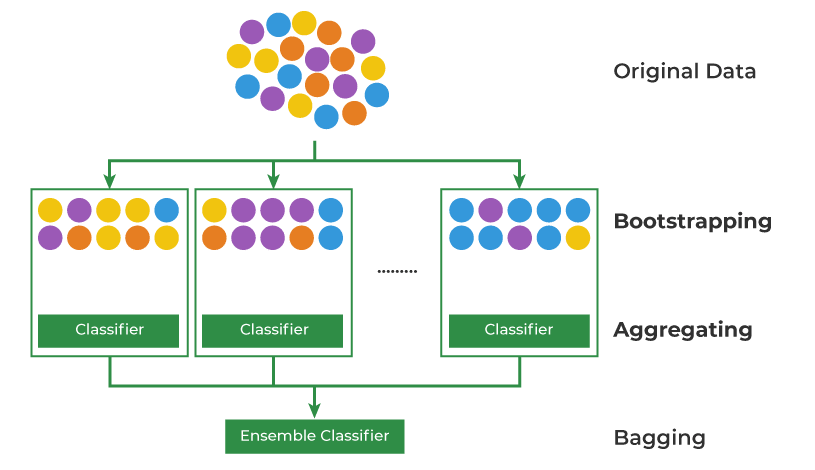
\includegraphics[width=0.8\textwidth]{Bagging-classifier.png}
\end{frame}

\begin{frame}{Bagging Algorithm}
    \textbf{Algorithm: Bagging (Bootstrap Aggregation)}
    
    \vspace{0.8em}
    
    \textbf{Input:} Training dataset $\mathcal{D} = \{(x_i, y_i)\}_{i=1}^{N}$, number of base models $B$
    
    \vspace{0.5em}
    \textbf{Output:} Final prediction $f_{\text{bag}}(x)$
    
    \vspace{0.5em}
    \begin{enumerate}
        \item For each $b = 1$ to $B$:
        \begin{itemize}
            \item Draw a bootstrap sample $\mathcal{D}_b$ of size $N$ from $\mathcal{D}$ (sampling with replacement)
            \item Train a base model $f_b(x)$ on $\mathcal{D}_b$
        \end{itemize}
        \item Compute the final prediction:
        \begin{itemize}
            \item \textbf{For classification:} Majority vote of $f_b(x)$
            \item \textbf{For regression:} Average of $f_b(x)$
        \end{itemize}
    \end{enumerate}
\end{frame}

\subsection{Random Forest}

\begin{frame}{Decision Trees in Bagging (Random Forest)}
    \textbf{Random Forest} is an ensemble learning method that builds multiple decision trees using the bagging (Bootstrap Aggregating) technique. Instead of training a single deep decision tree, Random Forest:
    \begin{itemize}
        \item Uses multiple decision trees as base models.
        \item Trains each tree on a random subset of data (bootstrap sampling).
        \item Selects a random subset of features at each split.
        \item Aggregates predictions using majority voting (classification) or averaging (regression).
    \end{itemize}
\end{frame}

\begin{frame}{Random Forest}
    \centering
    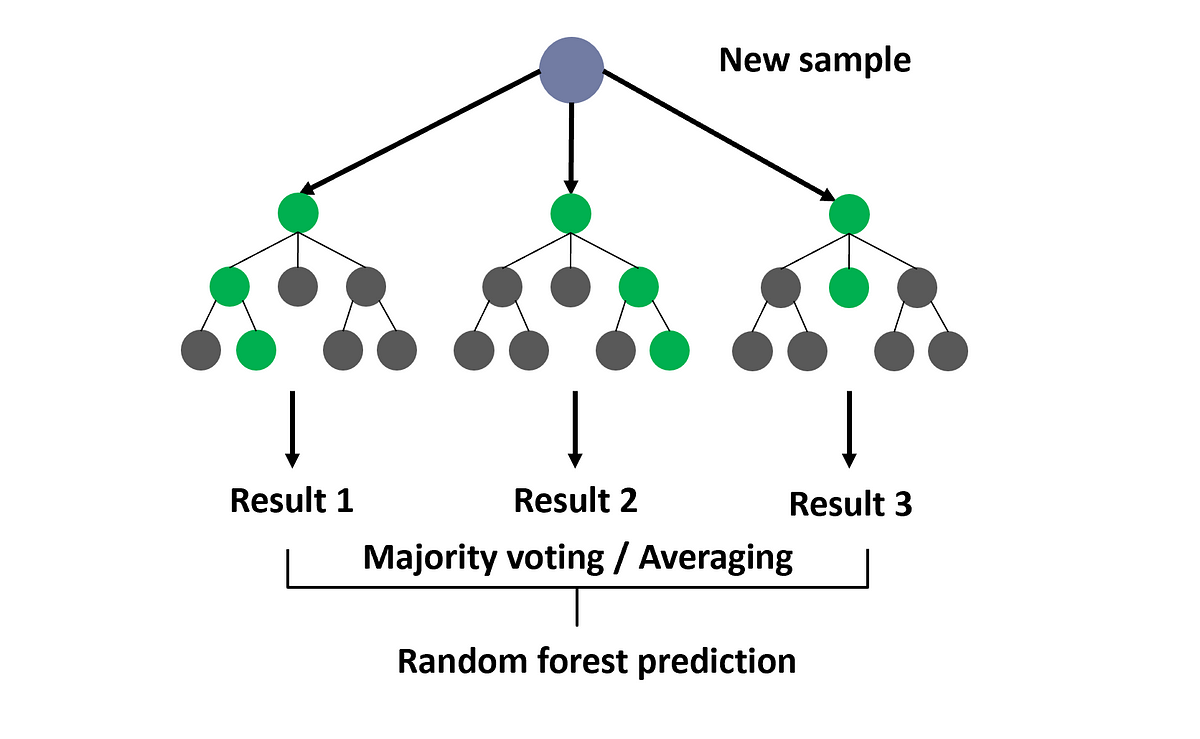
\includegraphics[width=0.8\textwidth]{randomforest.png}
\end{frame}

\begin{frame}{Random Forest Algorithm}
    \textbf{Steps:}
    \begin{enumerate}
        \item Select the number of trees \( B \) in the forest.
        \item For each tree \( b \):
        \begin{itemize}
            \item Draw a bootstrap sample \( D_b \) from dataset \( D \).
            \item Select a random subset of \( m \) features (usually \( m < \) total features).
            \item Grow a decision tree using \( D_b \) with selected features.
            \item Do not prune trees to keep them fully grown.
        \end{itemize}
        \item \textbf{For prediction:}
        \begin{itemize}
            \item \textbf{Classification:} Use majority voting across all trees.
            \item \textbf{Regression:} Use the average prediction from all trees.
        \end{itemize}
    \end{enumerate}
\end{frame}

\begin{frame}{Advantages of Random Forest}
    \begin{itemize}
        \item Reduces overfitting compared to a single decision tree.
        \item Handles high-dimensional data well.
        \item Works for both classification and regression tasks.
        \item Robust to missing data and noise.
        \item Provides feature importance ranking.
    \end{itemize}
\end{frame}

% Slide: Disadvantages
\begin{frame}{Disadvantages of Random Forest}
    \begin{itemize}
        \item Computationally expensive compared to a single decision tree.
        \item Less interpretable due to multiple trees.
        \item Requires careful tuning of hyperparameters (e.g., number of trees, number of features per split).
    \end{itemize}
\end{frame}


\begin{frame}
    \begin{center}
        {\Huge\ \color{red}For more information and code check the related notebook}
    \end{center}
\end{frame}

\begin{frame}
    \begin{center}
        {\Huge\ End of Ensemble Learning Part 1}
    \end{center}
\end{frame}

\end{document}

